\chapter{Concept and Model}\label{Chap:ProblemFormulation}



\section{Experimental Shock Tube IDT Uncertainty}
Every dataset in TUMKIN needs to contain appropriate uncertainties. If authors don't report uncertainties for experimental data, uncertainties are calculated using the Uncertainty Quantification(UQ) module of TUMKIN.
https://github.com/barkinguney/reaction-data-consistency-thesis

Reliable kinetic modeling and data-driven optimization require experimental databases with quantified uncertainties, yet more than 90\% of published ignition-delay time (IDT) datasets report none, which limits machine learning and statistical calibration. This work presents an automated algorithm to reconstruct uncertainty for shock-tube (ST) ignition-delay times when it is not reported in the original publication.

The method follows GUM and NIST guidance and separates uncertainty into systematic (Type-B) and random (Type-A) components. The combined standard uncertainty is defined as the square root of the sum of the squared systematic and random contributions, and the expanded uncertainty is reported with a coverage factor k=2 , corresponding to approximately 95\% confidence.

The systematic uncertainty captures device- and condition-specific biases in shock-tube IDT measurements and is treated as epistemic. Departures from an idealized zero-dimensional post-reflected-shock model are quantified by identifying dominant facility and operational non-idealities. Fourteen impacting factors describing hardware, operating conditions, diagnostics, and ignition-delay definition are selected to define proximity to an “ideal case.” A baseline systematic error of 5\% at 95\% confidence is assigned to this quasi-ideal reference.

Deviations from the ideal metrics are mapped to incremental penalties using a modified Harrington desirability function, which retains low sensitivity near the ideal point and saturation for large deviations. The individual penalties are aggregated to yield the total systematic uncertainty. This approach operationalizes systematic uncertainty in cases where rigorous multi-laboratory statistical evaluation is not feasible.

Random uncertainty is obtained by propagating uncertainties in input parameters, such as reflected-shock temperature, pressure, and equivalence ratio, through an analytical ignition-delay correlation using the law of uncertainty propagation. Manufacturer specifications, calibration data, or reasonable estimates are used when uncertainties are not explicitly reported.

The workflow outputs combined and expanded uncertainties with standardized and traceable bounds suitable for database integration. The method is demonstrated on published shock-tube datasets, where expanded combined uncertainties between approximately 15\% and 25\% are obtained, with the largest relative uncertainties occurring for very short and very long ignition delays.

The proposed procedure enables standardized uncertainty reporting for shock-tube IDTs and supports database ingestion, data-consistency analysis, Bayesian parameter estimation, and mechanism optimization. The implementation is prepared for integration into the developing TUMKIN chemical-kinetics cyber-infrastructure at the Technical University of Munich.

\begin{figure}[htbp]
	\centering
	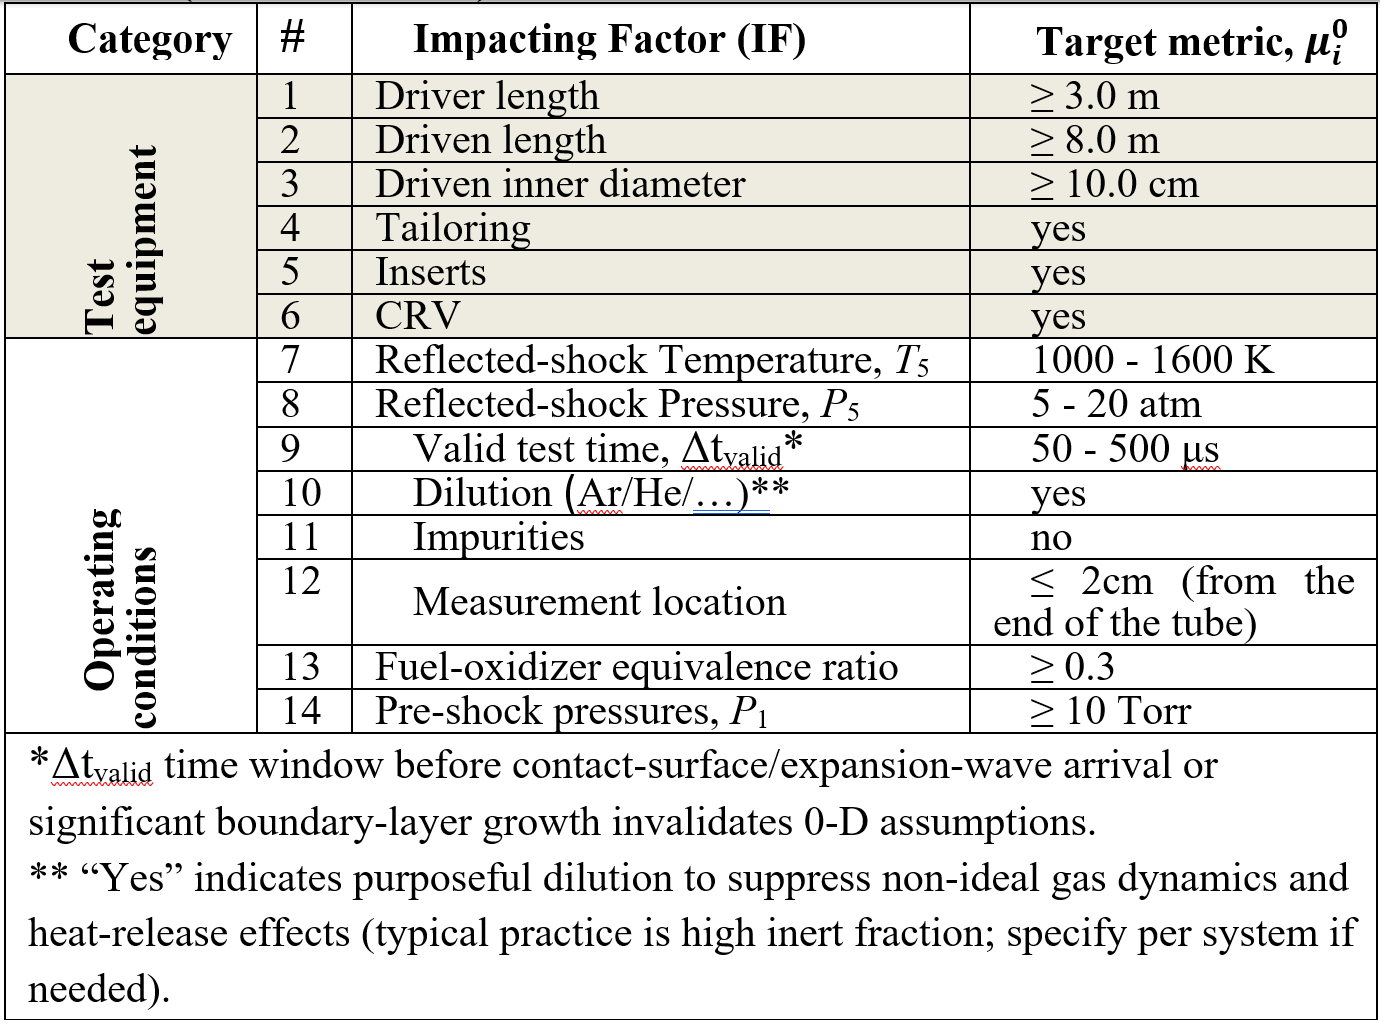
\includegraphics[width=0.8\textwidth]{Figures/impacting_factors.png}
	\caption{This is the description that appears under the image.}
	\label{fig:ifs}
\end{figure}


\begin{flalign}
	\begin{split}
		\sigma_i^2(\tau_{ign}) &= \left( z_2^C z_3^D A \exp \left( \frac{B}{z_1} \right) \cdot \left( -\frac{B}{z_1^2} \right) \right)^2 \cdot u^2(z_1) + \left( C A \exp \left( \frac{B}{z_1} \right) z_2^{C-1} z_3^D \right)^2 \cdot u^2(z_2) \\
		& + \left( D A \exp \left( \frac{B}{z_1} \right) z_2^C z_3^{D-1} \right)^2 \cdot u^2(z_3) + \left( \exp \left( \frac{B}{z_1} \right) z_2^C z_3^D \right)^2 \cdot u^2(A) \\
		& + \left( \frac{1}{z_1} A \exp \left( \frac{B}{z_1} \right) z_2^C z_3^D \right)^2 \cdot u^2(B) + \left( A \exp \left( \frac{B}{z_1} \right) z_2^C \ln(z_2) z_3^D \right)^2 \cdot u^2(C) \\
		& + \left( A \exp \left( \frac{B}{z_1} \right) z_2^C z_3^D \ln(z_3) \right)^2 \cdot u^2(D)
	\end{split} &
\end{flalign}

\section{Arrhenius Parameters Uncertainty}
Different sources report different values for the Arrhenius parameters or rate coefficients for the same reaction. Therefore, it is important to take all this information into account when analysing and optimizing reaction mechanisms. Kinetics databases like NIST chemical kinetics database and RMG database will be used to collect kinetics data, and calculate least squares fit to determine best parameters, and their distribution, specified by the covariance matrix of the least squares fit. Standard deviations of the parameters will be used to determine uncertainty bounds of the rate coefficients

\section{Cantera IDT Simulations}
Cantera is a 0D and 1D chemical kinetics software. To simulate shock tube IDT, constant volume batch reactors are used. Ignition delay times to be simulated for a given operating conditions T5, P5 phi and mechanism. The exact measurement or simulation time of IDT vary based on IDT definition.  Using the same IDT definition as reported by the physical experiment to calculate simulated IDT would yield the closest results to physical experiment. the The ignition types that can be handled by this IDT simulation code are a follow. Following the format described by RESPECTH shock tube IDT measurements, ignition type is comprised of attributes, target, type, amount and unit . Target can be pressure, temperature or concentration. Type can be “max”, “d/dt max”, “baseline max/min intercept from d/dt“, “concentration”, “relative concentration”, and “relative increase”. ”max” means IDT is at the maximum of the target property. “d/dt max” means IDT is at the maximum gradient of target property. “baseline max/min intercept from d/dt“ means the time when the max d/dt line intercepts the baseline value of target property. “concentration”: IDT is at the time target property reaches a specified concentration value. “relative concentration”: IDT is at the time when the concentration of the target property relative to its maximum concentration reach the specified value. “relative increase”:IDT is at the time when the value of  the target property increases by a given relative amount compared to its value at t=0.  Amount attribute is only used when type are “concentration”, “relative concentration” or “relative increase”. Unit attribute is only used when the type is  “concentration”, “relative concentration” or “relative increase”. Unit should have the value “unitless” for relative types. 
\section{Consistency analysis}
Consistency methods, that check for a given dataset of experimental ignition delay time measurements and a mechanism with parameter bounds, whether experiments and mechanism are consistent with each other.
\begin{figure}[htbp]
	\centering
	
\includegraphics[width=0.8\textwidth]{Figures/TUM_Logo_cmyk.pdf}
	\caption{Flowchart.}
	\label{fig:placeholder}
\end{figure}

\subsection{Sensitivity analysis}
For a given QoI, the model responses are sensitive to only a small subset of parameters. These parameters, referred to as active parameters, dominate the response behavior, a phenomenon referred to as effect sparsity [15]. Employing a sensitivity analysis method to identify these active parameters and using only these active parameters in further analysis improves computational feasibility. 
In [11] active parameters are identified by sampling the prior uncertainty region using space-filling designs like Latin hypercube sampling [16] or Sobol quasi-random sequence [17], and evaluating the original model at those points. A linear regression model Sl is then fitted to approximate the QoI as a function of the parameters.
\begin{equation}
	S_l = \sum_{i=1}^{n} c_i x_i + c_0
\end{equation}
$S_l$ contains information about how much the model output changes when each parameter is varied around its nominal value. 
The resulting regression coefficients define impact factors, which estimate how much the model output changes when each parameter varies across its uncertainty range. This is similar to sensitivity, but it also considers how large the parameter uncertainties are. A parameter with low sensitivity can still be high impact if it has high uncertainty. 
\begin{equation}
	\mathrm{IF}_i = \left|c_i\right| \,\left(u_i - l_i\right)
	= \left|c_i\right| \,\Delta x_i
\end{equation}
Active parameters are selected by screening the ranked impact factors with a preset threshold [11]. Depending on the use case sensitivity analysis or uncertainty analysis, $S_l$ or $\ \mathrm{I}Fi$ is used to rank parameters.






\section{Problem Formulation}





